\documentclass[12pt, twoside]{article}
\input{../preamble}

\fancyhead[LE]{\thepage}
\fancyhead[RO]{Solutions}
\fancyhead[LO]{La Scuola d'Italia / Dr.\ Huson / IB Math \\* 1 May 2026}

\begin{document}
\subsubsection*{11.15 Do Now: Introduction to Periodic Functions --- Solutions}

\begin{enumerate}[itemsep=0.4cm]

%--- Problem 1 ---
\item For $f(x) = 3\sin(2x) - 1$, comparing to $f(x) = a\sin(b(x+c)) + d$:
$a = 3$, $b = 2$, $c = 0$, $d = -1$.

\begin{enumerate}[itemsep=0.1cm]
  \item[(a)] amplitude $= |a| = 3$.
  \item[(b)] period $T = \dfrac{2\pi}{b} = \dfrac{2\pi}{2} = \pi$.
  \item[(c)] midline $y = d = -1$.
  \item[(d)] maximum value $= d + |a| = -1 + 3 = 2$.
\end{enumerate}

%--- Problem 2 ---
\item For $g(x) = 4\cos\!\left(\dfrac{\pi}{6}(x - 2)\right) + 5$, comparing to $g(x) = a\cos(b(x+c)) + d$ (with $c = -2$):
$a = 4$, $b = \dfrac{\pi}{6}$, $c = -2$, $d = 5$.

\begin{enumerate}[itemsep=0.1cm]
  \item[(a)] amplitude $= 4$.
  \item[(b)] period $T = \dfrac{2\pi}{\pi/6} = 12$.
  \item[(c)] midline $y = 5$.
  \item[(d)] $g$ is a maximum when the argument of $\cos$ is $0$ (or any multiple of $2\pi$). Setting
  $$\dfrac{\pi}{6}(x - 2) = 0 \quad\Longrightarrow\quad x = 2.$$
  Since $x = 2 \ge 0$, the smallest such $x$ is $\boxed{x = 2}$.
\end{enumerate}

%--- Problem 3: sketch of y = 2 sin x + 1 ---
\item $y = 2\sin x + 1$. \quad Amplitude $2$, period $2\pi$, midline $y = 1$.

\smallskip

Key features for the sketch:

\begin{itemize}[itemsep=0cm]
  \item $y$-intercept: $f(0) = 2\sin 0 + 1 = 1$.
  \item Maximum: $y = 1 + 2 = 3$ at $x = \dfrac{\pi}{2}$.
  \item Minimum: $y = 1 - 2 = -1$ at $x = \dfrac{3\pi}{2}$.
  \item Zero crossings (where $\sin x = -\tfrac{1}{2}$): $x = \dfrac{7\pi}{6}$ and $x = \dfrac{11\pi}{6}$.
\end{itemize}

\begin{center}
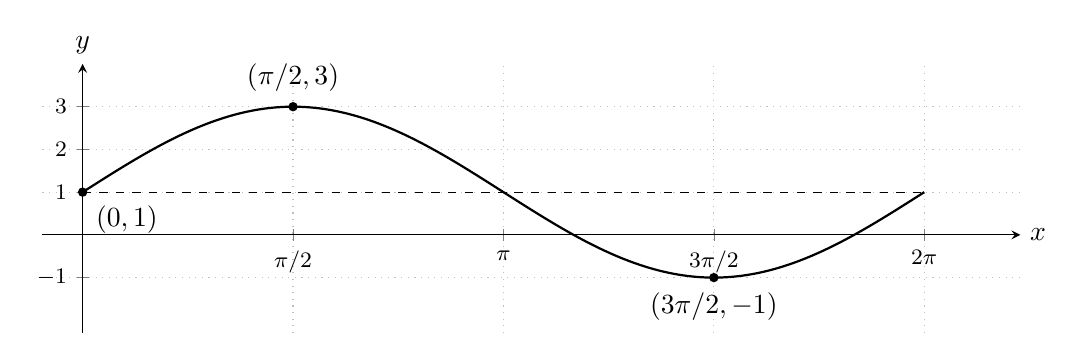
\begin{tikzpicture}
\begin{axis}[
    width=14cm, height=5cm,
    axis lines=middle,
    xlabel={$x$}, ylabel={$y$},
    xlabel style={at={(ticklabel* cs:1)}, anchor=west},
    ylabel style={at={(ticklabel* cs:1)}, anchor=south},
    xmin=-0.3, xmax=7,
    ymin=-2.3, ymax=4,
    xtick={1.5708, 3.1416, 4.7124, 6.2832},
    xticklabels={$\pi/2$, $\pi$, $3\pi/2$, $2\pi$},
    ytick={-1, 1, 2, 3},
    grid=major, grid style={dotted, gray!50},
    samples=200,
    tick label style={font=\footnotesize},
]
\addplot[thick, domain=0:6.2832] {2*sin(deg(x)) + 1};
\addplot[dashed, thin, domain=0:6.2832] {1};
\node[circle, fill=black, inner sep=1.2pt, label=above:{$(\pi/2, 3)$}] at (axis cs:1.5708,3) {};
\node[circle, fill=black, inner sep=1.2pt, label=below:{$(3\pi/2, -1)$}] at (axis cs:4.7124,-1) {};
\node[circle, fill=black, inner sep=1.2pt, label=below right:{$(0, 1)$}] at (axis cs:0,1) {};
\end{axis}
\end{tikzpicture}
\end{center}

%--- Problem 4: inverse problem ---
\item Given $f(x) = a\sin(b(x + c)) + d$ with $\max = 7$, $\min = 1$, period $T = 8$, and first maximum at $x = 1$.

\smallskip

\textit{Step 1 (amplitude and midline).}
$$a = \dfrac{\max - \min}{2} = \dfrac{7 - 1}{2} = 3, \qquad d = \dfrac{\max + \min}{2} = \dfrac{7 + 1}{2} = 4.$$

\textit{Step 2 (period factor).}
$$b = \dfrac{2\pi}{T} = \dfrac{2\pi}{8} = \dfrac{\pi}{4}.$$

\textit{Step 3 (phase from the first maximum).} \quad At a maximum, $\sin(b(x + c)) = 1$, so $b(x + c) = \dfrac{\pi}{2}$. Substituting $x = 1$:
$$\dfrac{\pi}{4}(1 + c) = \dfrac{\pi}{2} \quad\Longrightarrow\quad 1 + c = 2 \quad\Longrightarrow\quad c = 1.$$

\textit{Answer.} $\quad a = 3$, $\;b = \dfrac{\pi}{4}$, $\;c = 1$, $\;d = 4$. \quad That is,
$$f(x) = 3\sin\!\left(\dfrac{\pi}{4}(x + 1)\right) + 4.$$

\textit{Check.} $f(1) = 3\sin(\pi/2) + 4 = 7$ \checkmark; $\;f(5) = 3\sin(3\pi/2) + 4 = 1$ \checkmark (minimum half a period later).

\end{enumerate}
\end{document}
